	\section{Introduction: Beamer}

		\begin{frame}[fragile]{Title page}
			The Title page is printed using the command:			
			\begin{verbatim}    \maketitle\end{verbatim}
			
			The element printed on this page are defined in the preamble by
			\begin{verbatim}
				\title{Univ-Eiffel Template}
				\subtitle{A modern beamer theme based}
				\date{\today}
				\author[romain.noel@univ-eiffel.fr]{Romain NOËL}
				\institute{Universtity Gustave Eiffel}
				\titlegraphic{\hfill\includegraphics[height=1.5cm, draft]{Title_logo.pdf}}
				\logo{
\includegraphics[height=1.5cm, draft]{logo.pdf}}
			\end{verbatim}
		\end{frame}
		
		\begin{frame}[fragile]{Plain Slide}
			The usual page is printed and defined using the command:			
			\begin{verbatim}
				begin{frame}
				   \frametitle{Title on top of the frame}
				   contenu...
				end{frame}
			\end{verbatim}
			²
			Note that the logo printed on this page are defined in the preamble by
			\begin{verbatim}
				\logo{
\includegraphics[height=1.5cm, draft]{logo.pdf}}
			\end{verbatim}
		\end{frame}
	
		\begin{frame}[fragile]{Sections}
			Sections group slides of the same topic
			
			\begin{verbatim}    \section{Elements}\end{verbatim}
		\end{frame}
	
		\begin{frame}[fragile]{Typography}
			\begin{verbatim}
				The theme provides sensible defaults to
				\emph{emphasize} text, \alert{accent} parts
				or show \textbf{bold} results.
			\end{verbatim}
			
			\begin{center}becomes\end{center}
			
			The theme provides sensible defaults to \emph{emphasize} text,
			\alert{accent} parts or show \textbf{bold} results.
		\end{frame}
			
		\begin{frame}{Font feature test}
			\begin{itemize}
				\item Regular
				\item \textit{Italic}
				\item \textsc{Small Caps}
				\item \textbf{Bold}
				\item \textbf{\textit{Bold Italic}}
				\item \textbf{\textsc{Bold Small Caps}}
				\item \texttt{Monospace}
				\item \texttt{\textit{Monospace Italic}}
				\item \texttt{\textbf{Monospace Bold}}
				\item \texttt{\textbf{\textit{Monospace Bold Italic}}}
			\end{itemize}
		\end{frame}
			
		\begin{frame}{Lists}
			\begin{columns}[T,onlytextwidth]
				\column{0.33\textwidth}
					Items
					\begin{itemize}
					  \item Milk \item Eggs \item Potatoes
					\end{itemize}
				
				\column{0.33\textwidth}
					Enumerations
					\begin{enumerate}
					  \item First, \item Second and \item Last.
					\end{enumerate}
				
				\column{0.33\textwidth}
					Descriptions
					\begin{description}
					  \item[PowerPoint] Meeh. \item[Beamer] Yeeeha.
					\end{description}
			\end{columns}
			
			\vspace{1em}
			Then, something below the columns, that be long enough to recover all the line-width.
		\end{frame}
		
		\begin{frame}{Animation}
			\begin{itemize}%[<+- | alert@+>]
				\item \alert<4>{This is\only<4>{ really} important}
				\item Now this
				\item And now this
			\end{itemize}
		\end{frame}
		
		\begin{frame}{Figures}
			\begin{figure}
				\centering
				\newcounter{density}
				\setcounter{density}{20}
				\begin{tikzpicture}
					\def\couleur{alerted text.fg}
					\path[coordinate] (0,0)  coordinate(A)
					            ++( 90:5cm) coordinate(B)
					            ++(0:5cm) coordinate(C)
					            ++(-90:5cm) coordinate(D);
					\draw[fill=\couleur!\thedensity] (A) -- (B) -- (C) --(D) -- cycle;
					\foreach \x in {1,...,40}{%
					    \pgfmathsetcounter{density}{\thedensity+20}
					    \setcounter{density}{\thedensity}
					    \path[coordinate] coordinate(X) at (A){};
					    \path[coordinate] (A) -- (B) coordinate[pos=.10](A)
					                        -- (C) coordinate[pos=.10](B)
					                        -- (D) coordinate[pos=.10](C)
					                        -- (X) coordinate[pos=.10](D);
					    \draw[fill=\couleur!\thedensity] (A)--(B)--(C)-- (D) -- cycle;
					}
				\end{tikzpicture}
				\caption{Rotated square with Tikz package from
				\href{http://www.texample.net/tikz/examples/rotated-polygons/}{texample.net}.}
			\end{figure}
		\end{frame}
		
		\begin{frame}{Tables}
			\begin{table}
				\centering
				\caption{Largest cities in the world (source: Wikipedia)}
				\begin{tabular}{@{} lr @{}}
					\toprule
					City & Population\\
					\midrule
					Mexico City & 20,116,842\\
					Shanghai & 19,210,000\\
					Peking & 15,796,450\\
					Istanbul & 14,160,467\\
					\bottomrule
				\end{tabular}
			\end{table}
		\end{frame}
		
		
		\begin{frame}{Blocks}
			Three different block environments are pre-defined.
			
			\begin{block}{Default}
			  Block content.
			\end{block}
			
			\begin{alertblock}{Alert}
			  Block content.
			\end{alertblock}
			
			\begin{exampleblock}{Example}
			  Block content.
			\end{exampleblock}
		\end{frame}
		
		\begin{frame}{Math}
			\begin{equation}
				e = \lim_{n\to \infty} \left(1 + \frac{1}{n}\right)^n
			\end{equation}
		\end{frame}
		
		\begin{frame}{Line plots}
			\begin{figure}
				\centering
				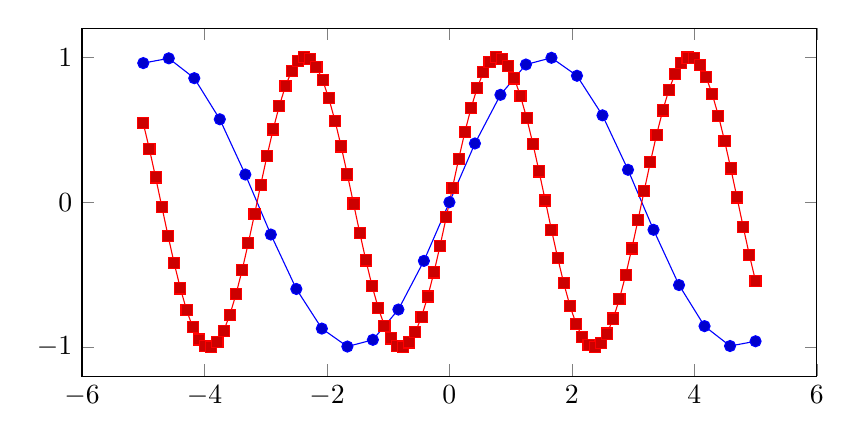
\begin{tikzpicture}
					\begin{axis}[
						width=0.9\textwidth,
						height=6cm,
						]
						
						\addplot {sin(deg(x))};
						\addplot+[samples=100] {sin(deg(2*x))};
					
					\end{axis}
				\end{tikzpicture}
				\caption{A nice sinus plot with Tikz.}
			\end{figure}
		\end{frame}
		
		\begin{frame}{Bar charts}
			\begin{figure}
				\centering
				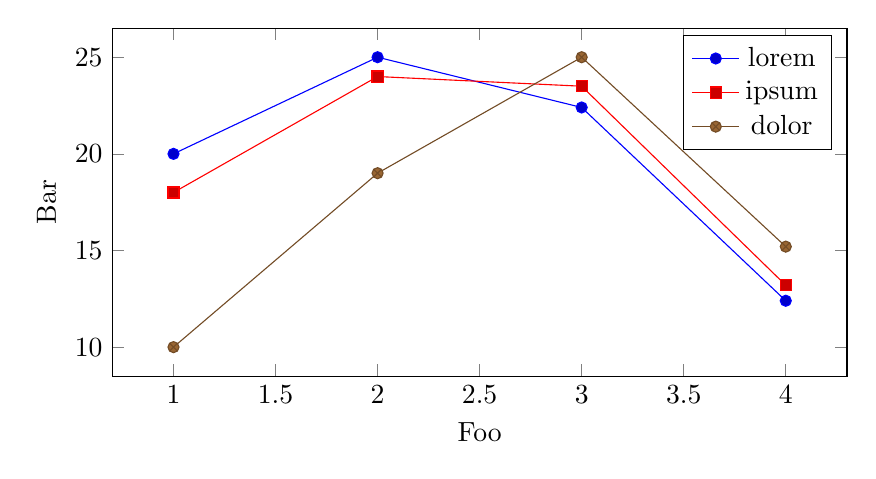
\begin{tikzpicture}
					\begin{axis}[
							xlabel={Foo},
						  	ylabel={Bar},
						  	width=0.9\textwidth,
						  	height=6cm,
						]
						
						\addplot plot coordinates {(1, 20) (2, 25) (3, 22.4) (4, 12.4)};
						\addplot plot coordinates {(1, 18) (2, 24) (3, 23.5) (4, 13.2)};
						\addplot plot coordinates {(1, 10) (2, 19) (3, 25) (4, 15.2)};
						
						\legend{lorem, ipsum, dolor}
					
					\end{axis}
				\end{tikzpicture}
				\caption{A nice bar chart with Tikz.}
			\end{figure}
		\end{frame}
		
		\begin{frame}{Quotes}
			\begin{quote}
				Veni, Vidi, Vici
			\end{quote}
			from Julius Caesar.
		\end{frame}
			
		\begin{frame}{References}
			Some references to showcase [allowframebreaks] \cite{Knuth92,ConcreteMath,Simpson,Er01,greenwade93}
		\end{frame}
	